% Сборка: cd docs/slides && latexmk -xelatex slides.tex
\documentclass[aspectratio=169,11pt]{beamer}
\usepackage{fontspec}
\setsansfont{Fira Sans}[Scale=0.95]
\setmainfont{Fira Sans}
\setmonofont{Fira Mono}[Scale=0.85]
\newfontfamily\cyrillicfont{Fira Sans}
\newfontfamily\cyrillicfontsf{Fira Sans}
\newfontfamily\cyrillicfonttt{Fira Mono}[Scale=0.85]
\usepackage{polyglossia}
\setdefaultlanguage{russian}
\setotherlanguage{english}
\usepackage{booktabs,tikz,graphicx,array}
\usetikzlibrary{arrows.meta,positioning,shapes.geometric,fit,backgrounds}

% ---- MIPT palette (measured on mipt.ru) ----
\definecolor{miptblue}{HTML}{003092}
\definecolor{miptmid}{HTML}{0A46C0}
\definecolor{mipttint}{HTML}{E6ECF9}
\definecolor{mipterr}{HTML}{B42318}
\definecolor{miptok}{HTML}{067647}
\definecolor{miptgrey}{HTML}{5B6B8C}

\usetheme{default}
\setbeamercolor{normal text}{fg=black}
\setbeamercolor{frametitle}{fg=miptblue}
\setbeamercolor{title}{fg=miptblue}
\setbeamercolor{structure}{fg=miptmid}
\setbeamercolor{itemize item}{fg=miptmid}
\setbeamerfont{frametitle}{series=\bfseries,size=\Large}
\setbeamertemplate{navigation symbols}{}
\setbeamertemplate{itemize items}[circle]
\setbeamertemplate{frametitle}{\vspace{6pt}\insertframetitle\par\vspace{-2pt}{\color{miptblue}\rule{\textwidth}{1.2pt}}}
\setbeamertemplate{footline}{\hfill{\color{miptgrey}\scriptsize Хакатон МФТИ · Задача 1\quad\insertframenumber\,/\,\inserttotalframenumber}\hspace*{10pt}\vspace{6pt}}
\newcommand{\bignum}[1]{{\color{miptblue}\bfseries\Huge #1}}
\newcommand{\muted}[1]{{\color{miptgrey}#1}}

\title{Проверка технического задания по 223-ФЗ}
\subtitle{находим, объясняем и исправляем ошибки в ТЗ на закупку}
\date{2026}

\begin{document}

% ---------------------------------------------------------------- 1
\begin{frame}[plain]
  \begin{tikzpicture}[remember picture,overlay]
    \fill[white] (current page.north west) rectangle ([yshift=-1.25cm]current page.north east);
    \fill[miptblue] ([yshift=-1.25cm]current page.north west) rectangle ([yshift=-1.35cm]current page.north east);
    \node[anchor=west] at ([xshift=0.8cm,yshift=-0.62cm]current page.north west) {
\includegraphics[height=0.75cm]{logo.pdf}};
    \node[anchor=east,text=miptgrey] at ([xshift=-0.8cm,yshift=-0.62cm]current page.north east) {\small Хакатон МФТИ · Задача 1};
    \node[anchor=north west, text=miptblue, font=\bfseries\fontsize{30}{34}\selectfont] at ([xshift=0.8cm,yshift=-2.0cm]current page.north west) {Проверка ТЗ · 223-ФЗ};
    \node[anchor=north west, text width=11cm, font=\Large] at ([xshift=0.8cm,yshift=-3.4cm]current page.north west) {находим, объясняем и исправляем ошибки в технических заданиях на закупку};
    \node[anchor=north west, text=miptblue, font=\bfseries\Huge] at ([xshift=0.8cm,yshift=-5.3cm]current page.north west) {27/27};
    \node[anchor=north west, text=miptgrey, text width=4.4cm, align=left, font=\small] at ([xshift=0.8cm,yshift=-6.4cm]current page.north west) {правок эксперта найдено};
    \node[anchor=north west, text=miptblue, font=\bfseries\Huge] at ([xshift=5.6cm,yshift=-5.3cm]current page.north west) {0};
    \node[anchor=north west, text=miptgrey, text width=4.4cm, align=left, font=\small] at ([xshift=5.6cm,yshift=-6.4cm]current page.north west) {ложных ошибок на исправленных ТЗ};
    \node[anchor=north west, text=miptblue, font=\bfseries\Huge] at ([xshift=10.4cm,yshift=-5.3cm]current page.north west) {32/32};
    \node[anchor=north west, text=miptgrey, text width=4.4cm, align=left, font=\small] at ([xshift=10.4cm,yshift=-6.4cm]current page.north west) {автоисправлений снимают замечание};
    \node[anchor=north west, text=miptmid, font=\ttfamily] at ([xshift=0.8cm,yshift=-7.7cm]current page.north west) {https://185-17-3-218.sslip.io};
  \end{tikzpicture}
\end{frame}

% ---------------------------------------------------------------- 2
\begin{frame}{Задача}
  \begin{columns}[T]
    \column{0.52\textwidth}
    На вход — техническое задание. На выход — результат, с которым сотрудник закупок может доработать документ:
    \begin{itemize}
      \item проблема и \textbf{конкретный фрагмент} ТЗ
      \item категория, \textbf{объяснение}, \textbf{исправление}
      \item ссылка на \textbf{норму}, без выдуманных оснований
      \item итоговое заключение
    \end{itemize}
    \vspace{6pt}
    \muted{Ограничение: наружу — только открытые данные.\\ Наше решение работает полностью локально.}
    \column{0.45\textwidth}
    \small
    \begin{tabular}{@{}l@{}}
      \toprule
      \textbf{Категории из брифа}\\ \midrule
      противоречие\\ некорректная характеристика\\ код ОКПД 2\\ гарантийные условия\\ стандарты\\ комплектность\\ ограничение конкуренции\\ \bottomrule
    \end{tabular}
  \end{columns}
\end{frame}

% ---------------------------------------------------------------- 3
\begin{frame}{Главный принцип: доказательства, а не мнение модели}
  \centering
  \begin{tikzpicture}[node distance=14mm and 6mm, box/.style={draw=miptmid, rounded corners=4pt, fill=mipttint, minimum height=13mm, text width=27mm, align=center, font=\small},
                      ar/.style={-{Stealth[length=2.4mm]}, thick, miptmid}]
    \node[box] (in) {ТЗ\\\scriptsize DOCX · PDF · DOC};
    \node[box, right=of in] (p) {Разбор\\\scriptsize разделы, таблицы, позиции};
    \node[box, right=of p] (c) {Проверки\\\scriptsize около 30 видов};
    \node[box, right=of c] (r) {Отчёт\\\scriptsize фрагмент, категория, норма};
    \node[box, below=of p, fill=miptblue!8, draw=miptblue] (k) {База знаний\\\scriptsize 223-ФЗ, ФАС, ОКПД2, ГОСТ};
    \node[box, below=of c, fill=white] (fb) {Отзывы\\\scriptsize обучение с проверкой};
    \node[box, below=of r, fill=miptok!10, draw=miptok] (f) {Автоисправление\\\scriptsize правило, ОКПД2, LLM};
    \draw[ar] (in) -- (p); \draw[ar] (p) -- (c); \draw[ar] (c) -- (r); \draw[ar] (r) -- (f);
    \draw[ar] (k) -- (c); \draw[ar] (fb) -- (c);
    \draw[ar] (f) -- (fb);
  \end{tikzpicture}
  \vspace{8pt}
  \begin{itemize}
    \item \textbf{Правила} находят дефект, \textbf{база знаний} даёт основание, \textbf{LLM} только формулирует — и её ответ проверяется
    \item Каждое исправление снова проходит проверки; отзывы и правки экспертов обучают систему
    \item Нет данных для вывода $\Rightarrow$ «требует проверки», а не «нарушение»
  \end{itemize}
\end{frame}

% ---------------------------------------------------------------- 4
\begin{frame}{Что проверяем}
  \small
  \begin{tabular}{@{}p{0.27\textwidth}p{0.68\textwidth}@{}}
    \toprule
    \textbf{Противоречия} & значение характеристики в таблице против предмета закупки и спецификации (тип лифта, грузоподъёмность, ОЗУ, площадь)\\
    \textbf{Характеристики} & число без единицы — с учётом смысла: «4 остановки» и «класс точности 0» единиц не требуют; оценочные слова\\
    \textbf{ОКПД 2} & несуществующий код, слишком общий «…190», код работ у товара, поставка без позиции с кодом товара\\
    \textbf{Гарантия} & основание начала срока против вида договора: товар — накладная, работы — КС-2/КС-3, услуги — акт\\
    \textbf{Стандарты} & «ГОСТ 53782-2010» без «Р» (реестр из 46\,752 пунктов реальных ТЗ)\\
    \textbf{Комплектность} & комплект без состава, разнородный комплект под одним кодом, позиция без характеристик\\
    \textbf{Конкуренция} & марка без «или эквивалент», запрет эквивалента, количественные требования к опыту\\
    \textbf{Вне ТЗ} & положения о национальном режиме и т.\,п., которым место в документации\\
    \bottomrule
  \end{tabular}
\end{frame}

% ---------------------------------------------------------------- 5
\begin{frame}{Как это выглядит}
  \centering
  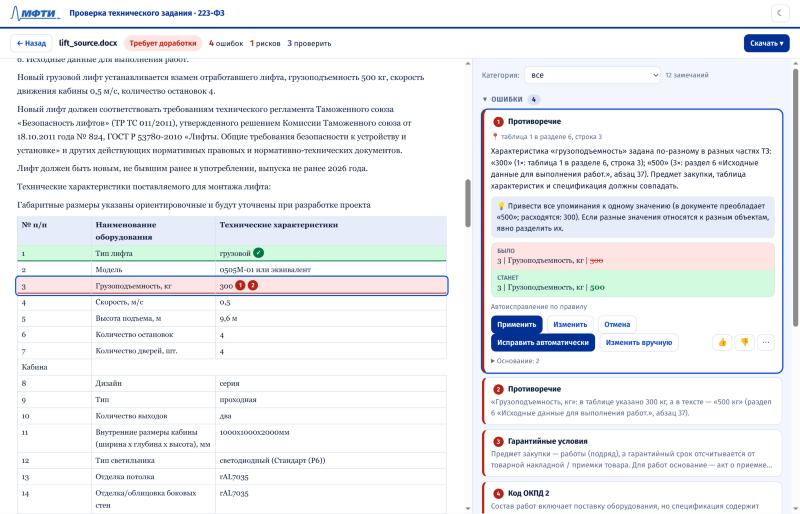
\includegraphics[width=0.92\textwidth]{../img/review_light.jpg}\\[3pt]
  \muted{\small Слева — документ с подсветкой, справа — замечания по группам. «Исправить автоматически»: было / станет, затем перепроверка.}
\end{frame}

% ---------------------------------------------------------------- 6
\begin{frame}{Автоисправление, которое проверяет само себя}
  \small
  \begin{tabular}{@{}>{\raggedright\arraybackslash}p{0.45\textwidth}>{\raggedright\arraybackslash}p{0.45\textwidth}@{}}
    \toprule
    \textbf{Было} & \textbf{Станет}\\ \midrule
    Тип лифта: \textcolor{mipterr}{пассажирский} & Тип лифта: \textcolor{miptok}{грузовой}\\
    ГОСТ 53782-2010 & ГОСТ \textcolor{miptok}{Р} 53782-2010\\
    гарантия с даты \textcolor{mipterr}{товарной накладной} & с даты \textcolor{miptok}{актов КС-2 и КС-3}\\
    температура воды не менее 40 & не менее 40 \textcolor{miptok}{°C}\\
    Lenovo ThinkPad T14 Gen 4 & Lenovo ThinkPad T14 Gen 4 \textcolor{miptok}{или эквивалент}\\
    плита поверочная, 26.51.33.\textcolor{mipterr}{190} & 26.51.33.\textcolor{miptok}{142} — как у эксперта\\
    105 календарных дней & 105 \textcolor{miptok}{(Сто пять)} календарных дней\\ \bottomrule
  \end{tabular}
  \vspace{8pt}
  \begin{columns}[T]
    \column{0.62\textwidth}
    \begin{itemize}
      \item правила по виду замечания, подбор ОКПД2 по наименованию (TF-IDF по 21\,081 коду), LLM — запасной путь
      \item исправление \textbf{предлагается, только если повторная проверка его принимает}; применяется после подтверждения
    \end{itemize}
    \column{0.34\textwidth}
    \bignum{32/32}\ \muted{сняли замечание}\\[2pt]
    \bignum{0}\ \muted{новых проблем}
  \end{columns}
\end{frame}

% ---------------------------------------------------------------- 7
\begin{frame}{Качество на эталонах}
  \begin{columns}[T]
    \column{0.56\textwidth}
    \small
    \begin{tabular}{@{}>{\raggedright\arraybackslash}p{0.6\linewidth}cc@{}}
      \toprule
      \textbf{Документ} & \textbf{обяз.} & \textbf{доп.}\\ \midrule
      Лифт, работы & 6/6 & 2/2\\
      Метрология, поставка & 4/4 & 2/2\\
      Клининг, услуги (наш) & 9/9 & 2/2\\
      ИТ-техника (наш) & 8/8 & 1/1\\ \midrule
      \textbf{Итого} & \textbf{27/27} & \textbf{7/7}\\ \bottomrule
    \end{tabular}\\[8pt]
    Исправленные экспертом версии: \textbf{0} ложных ошибок.\\
    Облегчённый режим без PyTorch даёт тот же результат.
    \column{0.4\textwidth}
    \small
    \textbf{Как меряем}
    \begin{itemize}
      \item правки эксперта (исходное $\to$ итоговое) переведены в эталонные замечания
      \item полнота — на исходных ТЗ, ложные ошибки — на итоговых
      \item два собственных ТЗ из других областей проверяют, что логика не подогнана под примеры
      \item всё воспроизводится: \texttt{eval\_case.py}, \texttt{eval\_autofix.py}
    \end{itemize}
  \end{columns}
\end{frame}

% ---------------------------------------------------------------- 8
\begin{frame}{Данные и модели}
  \begin{columns}[T]
    \column{0.48\textwidth}
    \small\textbf{Собрали сами}
    \begin{itemize}
      \item ЕИС: 321 закупка, 2\,778 вложений, 46\,752 пункта ТЗ
      \item ФАС: 437 дел, 692 решения, 420 доводов
      \item 223-ФЗ и 44-ФЗ: 1\,623 нормы по частям, 76 изменяющих законов
      \item ОКПД2: 21\,081 код
    \end{itemize}
    \column{0.48\textwidth}
    \small\textbf{Модели (все локальные)}
    \begin{itemize}
      \item RuBERT-tiny2, дообучен: роль пункта (29\,M параметров, 7 мин на CPU)
      \item multilingual-e5-small: поиск норм и решений ФАС
      \item Qwen2.5-7B, 4 бит: пояснения; ответ проверяется на выдуманные нормы и числа
      \item фильтр замечаний, обучаемый на отзывах экспертов
    \end{itemize}
  \end{columns}
  \vspace{6pt}
  \muted{\small Почему не «просто LLM»: первая же 7B-модель переписала «не менее 7» в «ровно 7» и придумала марку стали.}
\end{frame}

% ---------------------------------------------------------------- 9
\begin{frame}{Учится на работе экспертов}
  \begin{itemize}
    \item каждое замечание: \textbf{«верно» / «ложное»}, «другая категория», комментарий; клик по тексту — «система пропустила проблему»
    \item каждая правка: исходный текст, предложение системы, итоговый текст, сняло ли замечание
    \item датасеты собираются автоматически; фильтр переобучается в фоне
    \item \textbf{ворота качества}: новая модель включается, только если на эталонах не теряет ни одной обязательной правки и не добавляет ложных
  \end{itemize}
  \vspace{6pt}
  \small
  \begin{tabular}{@{}>{\raggedright\arraybackslash}p{0.2\textwidth}>{\raggedright\arraybackslash}p{0.5\textwidth}>{\raggedright\arraybackslash}p{0.24\textwidth}@{}}
    \toprule
    Проверка ворот & Отзывы & Решение\\ \midrule
    полезные отзывы & эксперты отклоняют замечания об оформлении & \textcolor{miptok}{включена}\\
    вредные отзывы & «отклоняют» настоящие противоречия & \textcolor{mipterr}{отклонена} (27 $\to$ 17)\\ \bottomrule
  \end{tabular}
\end{frame}

% ---------------------------------------------------------------- 10
\begin{frame}{Развёртывание}
  \begin{columns}[T]
    \column{0.5\textwidth}
    \small
    \begin{itemize}
      \item Docker + Docker Compose; один скрипт для VPS: Docker, HTTPS (Let's Encrypt), вход
      \item облегчённый режим для слабых серверов: 1 vCPU, 709 МБ RAM, 120 МБ на приложение
      \item вход: демо-режим, Яндекс ID, Google; доступ можно ограничить доменом \texttt{phystech.edu}
      \item никаких внешних API при проверке
    \end{itemize}
    \vspace{4pt}
    {\ttfamily\scriptsize ./deploy/deploy.sh root@HOST}
    \column{0.46\textwidth}
    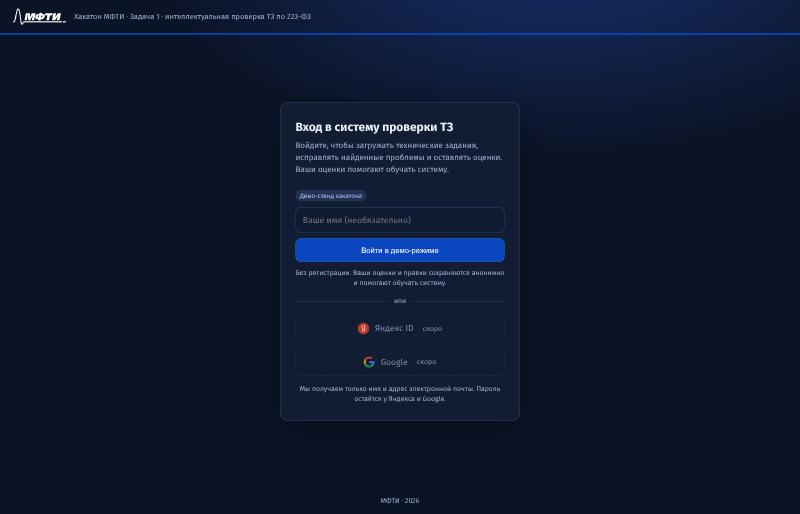
\includegraphics[width=\textwidth]{../img/login.jpg}
  \end{columns}
\end{frame}

% ---------------------------------------------------------------- 11
\begin{frame}{Ограничения и план}
  \begin{columns}[T]
    \column{0.48\textwidth}
    \textbf{Честно о границах}
    \small
    \begin{itemize}
      \item нет Положений о закупке заказчиков и перечня СМП — такие места помечены «требует проверки»
      \item нет рыночных каталогов: избыточность параметров — по признакам
      \item LLM на CPU медленная; на слабом сервере работает без неё
    \end{itemize}
    \column{0.48\textwidth}
    \textbf{Дальше}
    \small
    \begin{itemize}
      \item Положения о закупке из ЕИС $\to$ проверка по внутренним регламентам
      \item разметка 100 решений ФАС экспертами $\to$ обученные классификаторы вместо правил
      \item один класс товаров с каталогом рынка $\to$ проверка избыточности по данным
      \item исправления экспертов $\to$ дообучение LLM (LoRA)
    \end{itemize}
  \end{columns}
\end{frame}

% ---------------------------------------------------------------- 12
\begin{frame}[plain]
  \centering
  \vspace{1.4cm}
  {\color{miptblue}\bfseries\Huge Попробуйте сами\par}
  \vspace{10pt}
  {\Large\color{miptmid}\ttfamily https://185-17-3-218.sslip.io\par}
  \vspace{6pt}
  \muted{«Войти в демо-режиме» $\to$ любой пример документа $\to$ «Исправить автоматически»}
  \vspace{20pt}

  \begin{columns}[T]
    \column{0.3\textwidth}\centering\bignum{27/27}\\\muted{правок эксперта}
    \column{0.3\textwidth}\centering\bignum{0}\\\muted{ложных ошибок}
    \column{0.3\textwidth}\centering\bignum{1–3 с}\\\muted{на документ}
  \end{columns}
\end{frame}

\end{document}
